\documentclass[a4paper,11pt]{jsarticle}


% 数式
\usepackage{amsmath,amsfonts}
\usepackage{bm}
\usepackage{physics}
% 画像
\usepackage[dvipdfmx]{graphicx}
% ローマ数字
\usepackage{otf}
% 単位
\usepackage{siunitx}
% 表
\usepackage{multirow}
% 化学反応
\usepackage[version=4]{mhchem}

\usepackage{url}

\begin{document}

\title{固体物理学\ajRoman{3} 前半レポート}
\author{05-211525 齋藤駿一}
\date{\today}
\maketitle

\section*{問1 ハバードモデル}
\subsection*{(1)}
$i$番目($i=1,\cdots,n$)のサイトの位置を$r_i$とおくと,消滅演算子のフーリエ変換は
\begin{equation}
  c_{i\sigma} = \frac{1}{\sqrt{n}}\int \dd{k} e^{ik\cdot r_i} c_{k\sigma} 
\end{equation}
と書ける.
これとこの共役より,$U=0$のときのハミルトニアン$H_0$は
\begin{align}
  H_0 &= -t \sum_{\langle i,j\rangle,\sigma}\left(c^{\dagger}_{i\sigma}c_{j\sigma} + c^{\dagger}_{j\sigma}c_{i\sigma}\right)\notag\\
  &= -\frac{t}{n} \int \dd{k} \int \dd{k'} \sum_{\langle i,j\rangle,\sigma} \left(e^{ik'\cdot r_j - ik\cdot r_i} + e^{ik'\cdot r_i - ik\cdot r_j}\right) c^{\dagger}_{k\sigma} c_{k'\sigma} \notag\\
  &= -\frac{t}{n} \int \dd{k} \int \dd{k'} \sum_{\langle i,j\rangle,\sigma} \left(e^{i(k'-k)\cdot r_i}e^{ik'\cdot (r_j - r_i)} + e^{i(k'-k)\cdot r_i} e^{-ik\cdot (r_j - r_i)}\right) c^{\dagger}_{k\sigma} c_{k'\sigma} \notag
\end{align}
と書ける.
いま,格子定数$a$の2次元正方格子を考えているので,
\begin{align}
  H_0 &= -\frac{t}{n} \int \dd{k} \int \dd{k'} \sum_{i,\sigma} \left(e^{i(k'-k)\cdot r_i}\left(e^{ik'_xa} + e^{ik'_ya} \right)+ e^{i(k'-k)\cdot r_i} \left(e^{-ik'_xa} + e^{-ik'_ya} \right)\right) c^{\dagger}_{k\sigma} c_{k'\sigma}\notag\\
  &= - \frac{t}{n} \sum_{\sigma}\int \dd{k} \int \dd{k'} n\delta(k-k')\left(e^{ik'_xa} + e^{ik'_ya}+ e^{-ik'_xa} + e^{-ik'_ya} \right) c^{\dagger}_{k\sigma} c_{k'\sigma} \notag\\
  &= -t\sum_{\sigma}\int \dd{k} (2\cos{k_xa}+2\cos{k_ya})c^{\dagger}_{k\sigma} c_{k\sigma}
\end{align}
ここで,デルタ関数のフーリエ変換の公式を用いた.
したがって,波数$k$に対応するエネルギーは
\begin{equation}
  \epsilon_k = -2t(\cos{k_xa}+\cos{k_ya}) \label{eps_k}
\end{equation}
となる.

\subsection*{(2)}

\begin{figure}[htbp]
  \centering
  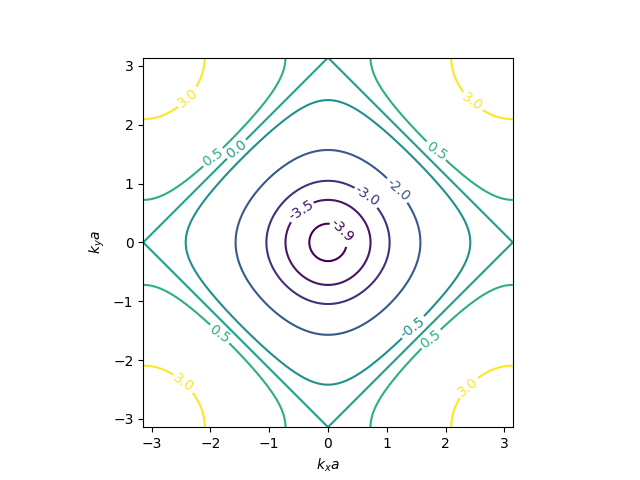
\includegraphics[width=13cm]{2DHM.png}
  \caption{$\epsilon_k/t$の等高線(値は線の上に記載した).等高線の形状は,バンドの底付近($\epsilon_k/t = -0.39,-0.35,0.30$)では円形に近く,バンドの中央付近($\epsilon_k/t=-0.5,0,0.5$)では正方形に近い.}
  \label{fig:2DHM}
\end{figure}

\subsubsection*{(i)バンドの底付近}
バンドの底付近では,$|k_x|a, |k_y|a \ll 1$が成り立つので,
\begin{equation}
  \epsilon_k \approx -2t(1-\frac{k_x^2a^2}{2}+1-\frac{k_y^2a^2}{2}) = -4t + tk^2a^2 
\end{equation}
より,等エネルギー線は円
\begin{equation}
  k = \mathrm{const.}
\end{equation}
で与えられる(図\ref{fig:2DHM}).

\subsubsection*{(ii)バンドの中間付近}
バンドの中間付近では,
\begin{equation}
  \cos{k_xa}+\cos{k_ya} = 2\cos{\left(\frac{k_x + k_y}{2}a\right)}\cos{\left(\frac{k_x - k_y}{2}a\right)} \approx 0
\end{equation}
が成り立つ.
とくに,バンドのちょうど中間では,
\begin{equation}
  k_x + k_y = \pm\frac{\pi}{a}, \qquad k_x - k_y = \pm\frac{\pi}{a}
\end{equation}
のいずれかが成り立つ.
つまり,バンドのちょうど中間の等エネルギー線は,第一ブリルアンゾーンの境界と$k_x,k_y$軸が交わる4点を結んだ正方形で与えられる.
その近傍のバンドの等エネルギー線は,概ねこの正方形に沿った曲線となる(図\ref{fig:2DHM}).

\subsection*{(3)}
式\eqref{eps_k}より,
\begin{equation}
  \left| \nabla_{k} \epsilon_k \right|
  = \left|-2t\left(
  \begin{array}{c}
    -a\sin{k_x a} \\
    -a\sin{k_y a}
  \end{array}
  \right)\right| 
  = 2ta \sqrt{\sin^2{k_x a}+\sin^2{k_x a}}
\end{equation}
である.

\subsubsection*{(i)バンドの底付近}
バンドの底付近では,$|k_x|a, |k_y|a \ll 1$より
\begin{equation}
  \left| \nabla_{k} \epsilon_k \right|  = 2ta \sqrt{\sin^2{k_x a}+\sin^2{k_x a}}\approx 2ta \sqrt{k_x^2a^2 + k_y^2a^2} = 2ta^2k
\end{equation}
と近似できる.
これと,(前問より)バンドの底付近の等エネルギー線$\epsilon_k=\epsilon$上では$k$を一定と見なせることから,状態密度は
\begin{align}
  D(\epsilon) &= \left(\frac{a}{2\pi}\right)^2 \oint_{\epsilon_k = \epsilon} \frac{dl}{\left| \nabla_{k} \epsilon_k \right|} \notag\\
  &\approx \left(\frac{a}{2\pi}\right)^2 \oint_{\epsilon_k = \epsilon} \frac{dl}{2ta^2k} \notag\\
  &\approx  \left(\frac{a}{2\pi}\right)^2 \frac{2\pi k}{2ta^2k} \notag\\
  &= \frac{1}{4\pi t}
\end{align}
と$\epsilon$によらない一定値をとる.

\subsubsection*{(ii)バンドの中間付近}


\subsection*{(4)}


\subsection*{(5)}
以降では,$H_0$に加えて相互作用項($U\neq 0$)
\begin{equation}
  H_1 = U \sum_i n_{i\uparrow} n_{i\downarrow}
\end{equation}
をハートリー・フォック近似で取り入れる.
まず,$n_{i\updownarrow}$を平均値とそこからのずれに分解し,
\begin{equation}
  n_{i\updownarrow} = \langle n_{i\updownarrow} \rangle + \left(n_{i\updownarrow} - \langle n_{i\updownarrow} \rangle\right)
\end{equation}
と書く.
次に,平均からのずれを微小量として2次以降を無視すると,
\begin{align}
  n_{i\uparrow} n_{i\downarrow} 
  &\approx \langle n_{i\uparrow} \rangle \langle n_{i\downarrow} \rangle 
  + \langle n_{i\uparrow} \rangle \left(n_{i\downarrow} - \langle n_{i\downarrow} \rangle\right)
  + \langle n_{i\downarrow} \rangle \left(n_{i\uparrow} - \langle n_{i\uparrow} \rangle\right)\notag\\
  &= \langle n_{i\downarrow} \rangle n_{i\uparrow} + \langle n_{i\uparrow} \rangle n_{i\downarrow} - \langle n_{i\uparrow} \rangle \langle n_{i\downarrow} \rangle  \notag\\
  &= \left(\frac{n}{2}-\alpha_{i}s\right)n_{i\uparrow} + \left(\frac{n}{2}+\alpha_{i}s\right)n_{i\downarrow} - \left(\frac{n^2}{4} - \alpha_i^2 s^2\right)
\end{align}
よって,相互作用項は
\begin{align}
  H_1 &= \sum_i \left[ \left(\frac{n}{2}-\alpha_{i}s\right)n_{i\uparrow} + \left(\frac{n}{2}+\alpha_{i}s\right)n_{i\downarrow} - \left(\frac{n^2}{4} - \alpha_i^2 s^2\right) \right] \notag\\
  &= \sum_i \left[ \left(\frac{n}{2}-\alpha_{i}s\right)n_{i\uparrow} + \left(\frac{n}{2}+\alpha_{i}s\right)n_{i\downarrow} \right] - \frac{n^3}{4} + ns^2
\end{align}
となる.
したがって,定数項を省くと,ハートリー・フォック近似のハミルトニアンは
\begin{equation}
  H_{\mathrm{HF}} = -t \sum_{\langle i,j\rangle,\sigma}\left(c^{\dagger}_{i\sigma}c_{j\sigma} + c^{\dagger}_{j\sigma}c_{i\sigma}\right) + \sum_i \left[ \left(\frac{n}{2}-\alpha_{i}s\right)n_{i\uparrow} + \left(\frac{n}{2}+\alpha_{i}s\right)n_{i\downarrow} \right]
\end{equation}
となる.

\subsection*{(6)}
相互作用項のフーリエ変換を考える.
まず,
\begin{align}
  n_{i\sigma} &= c^{\dagger}_{i\sigma}c_{i\sigma} \notag\\
  &= \frac{1}{n} \int \dd{k} e^{-ik\cdot r_i} c^{\dagger}_{k\sigma} \int \dd{k'} e^{ik'\cdot r_i} c_{k'\sigma} \notag\\
  &= \frac{1}{n} \int \dd{k} \int \dd{k'} e^{i(k'-k)\cdot r_i} c^{\dagger}_{k\sigma}c_{k'\sigma}
\end{align}
より,
\begin{align}
  \sum_i \frac{n}{2}\left(n_{i\uparrow} + n_{\downarrow}\right) 
  &= \frac{n}{2}\cdot\frac{1}{n} \int \dd{k} \int \dd{k'} \sum_i e^{i(k'-k)\cdot r_i}  \left(c^{\dagger}_{k\uparrow}c_{k'\uparrow} + c^{\dagger}_{k\downarrow}c_{k'\downarrow} \right)\notag\\
  &= \frac{n}{2} \int \dd{k} \left(c^{\dagger}_{k\uparrow}c_{k\uparrow} + c^{\dagger}_{k\downarrow}c_{k\downarrow}\right) \notag\\
  &= \frac{n}{2} \int \dd{k} \left(n_{k\uparrow} + n_{k\downarrow}\right)
\end{align}
が分かる.
一方,反強磁性ベクトル$Q$を用いて$\alpha_i = e^{iQ\cdot r_i}$と表すと,
\begin{align}
  \sum_i \alpha_i \left(n_{i\uparrow} - n_{i\downarrow}\right)
  &= s \frac{1}{n} \int \dd{k} \int \dd{k'}\sum_i e^{i(k'-k+Q)\cdot r_i} \left(c^{\dagger}_{k\uparrow}c_{k'\uparrow} - c^{\dagger}_{k\downarrow}c_{k'\downarrow} \right) \notag \\
  &= s \int \dd{k} \left(c^{\dagger}_{k\uparrow}c_{(k-Q)\uparrow} - c^{\dagger}_{k\downarrow}c_{(k-Q)\downarrow} \right) 
\end{align}
と書ける.
よって,
\begin{align}
  H_{\mathrm{HF}} &= \sum_{\sigma}\int \dd{k} \epsilon_k c^{\dagger}_{k\sigma} c_{k\sigma} + \frac{n}{2} \int \dd{k} \left(n_{k\uparrow} + n_{k\downarrow}\right) - s \int \dd{k} \left(c^{\dagger}_{k\uparrow}c_{(k-Q)\uparrow} - c^{\dagger}_{k\downarrow}c_{(k-Q)\downarrow} \right) \notag\\
  &= \int \dd{k} \left[\left(\epsilon_k + \frac{n}{2}\right) \left(n_{k\uparrow}+n_{k\downarrow}\right) - s \left(c^{\dagger}_{k\uparrow}c_{(k-Q)\uparrow} - c^{\dagger}_{k\downarrow}c_{(k-Q)\downarrow} \right)\right]
\end{align}
とフーリエ変換できる.

次に,ネスティング条件$\epsilon_k = - \epsilon_{k+Q}$を確認する.
いま,
\begin{equation}
  e^{iQ_x a} = e^{iQ_y a} = -1
\end{equation}
となるような$Q$を選んだので,この式の実部と虚部それぞれを\eqref{eps_k}に当てはめると,
\begin{equation}
  \epsilon_{k+Q} = -2t(\cos{(k_x+Q)a}+\cos{(k_y+Q)a}) = 2t(\cos{k_xa}+\cos{k_ya}) = -\epsilon_k
\end{equation}
が分かる.

\subsection*{(7)}


\section*{問2 論文まとめ}

\subsection*{論文の概要}
論文として,Cucchietti F.M.ら(2006)による``Dynamics of the Bose-Hubbard model: transition from Mott insulator to superfluid"を選んだ(下記URLから入手できる).

\begin{center}
  \url{https://arxiv.org/abs/cond-mat/0601650}
\end{center}

この論文は,1次元ボース・ハバードモデルにおける,モット絶縁体から超流動状態への転移を数値計算を用いて考察したものである.
2サイトモデルの場合には厳密解が知られているが,一般的な$M$サイトの場合のダイナミクスはよく分かっていない.
そこで,この論文は$M=3,\cdots,10$の数値計算を行い,そこで見られた性質を理論的に説明した.
とくに,速いダイナミクスについては(1)時間に依存する摂動論,(2)ボゴリューボフ理論を用い,遅いダイナミクスについては(3)キッブル・ズレック機構を用いて説明した.

\subsection*{代表的な図の解説の準備}
この論文で扱うボース・ハバードモデルとは,
\begin{equation}
  H = -J \sum_{i=1}^{M} \left(\hat{a}^{\dagger}_{i+1} \hat{a}_i + \mathrm{h.c.}\right) + \frac{1}{2}\sum_{i=1}^{M} \hat{n}_i \left(\hat{n}_i - 1\right)
\end{equation}
のことである.
第1項は隣接サイト間の飛び移り,つまり運動エネルギーであり,第2項は同じサイトを複数の粒子が占有した際の斥力ポテンシャルである.
なお,周期境界条件を仮定する.

転移を起こす際,$J$を時刻とともに
\begin{equation}
  J(t) = \frac{t}{\tau_Q}
\end{equation}
と変え,$J\gg 1$となったとき変化を止めるようにする.
モット絶縁体から超流動状態への転移の臨界点は$J\approx 0.29$にあるので,この$J$の変化により転移が起こる.
ここで,$\tau_Q$はクエンチの時定数を表す.

この論文が注目するのは,相関関数
\begin{equation}
  C_l(t) = \frac{1}{2} \ev{\hat{a}^{\dagger}_{i+l} \hat{a}_i + \mathrm{h.c.}}{\psi (t)}
\end{equation}
である.
$J$が大きくなるにつれて,この値は増大する.

まず,2サイトモデル($M=2$)の場合を考えると,解析的に$C_1(\infty)$の厳密解が得られる.
とくに,$\tau_Q$が小さいとき
\begin{equation}
  C_1 (\infty) = \frac{\sqrt{\pi}}{4}\sqrt{\tau_Q} + \mathcal{O}\left(\tau_Q^{3/2}\right)
\end{equation}
と展開でき,$\tau_Q$が大きいとき
\begin{equation}
  C_1 (\infty) = 1 - \frac{8}{\tau_Q^2} + \mathcal{O}\left(\tau_Q^{-4}\right)
\end{equation}
と展開できる.

この論文では,$\tau_Q$が小さい場合と大きい場合に分けて,$M>2$のモデルについて議論していた.
しかし,$\tau_Q$が大きい場合については図がなかったので,ここでは$\tau_Q$が小さい場合だけ取り上げる.

\subsection*{代表的な図の解説}

まず,著者らは$M=3,\cdots,10$の場合について数値計算を行い,$\tau_Q < 10^{-1}$の場合には
\begin{equation}
  C_1(\infty) = \alpha \tau_Q^{\beta}
\end{equation}
でフィッティングでき,
\begin{equation}
  \alpha \in (0.37,0.5),\qquad \beta \approx \frac{1}{2}
\end{equation}
であることを見いだした.
つまり,$M=2$での厳密解は,$M=3,\cdots,10$でも近似的に成り立っているといえる.
たとえば,$M=10$のときのフィッティングは図\ref{fig:paper_1}の内側の図のようになる.

さらに$\tau_Q < 0.1$では,図\ref{fig:paper_1}の外側の図のように,$C_1(t)$の形状は
\begin{equation}
  C_1(t) \to \frac{C_1\left(\frac{t}{\sqrt{\tau_Q}}\right)}{\sqrt{\tau_Q}}
\end{equation}
というリスケーリングに関して不変であることも分かった.
著者らは,これが成り立つかを実験で検証するのは興味深いと述べていた.
実際,上述したフィッティングが当てはまる$\tau_Q = 10^{-1}$で,$C_1(\infty)\approx 0.16$となっており(図\ref{fig:paper_1}),これは超流動への転移点での値($C_1(\infty)\approx 0.8$)や超流動状態での値($C_1(\infty) = 1$)と比べてそこまで小さくないため,実験的に測定できる.

\begin{figure}[htbp]
  \centering
  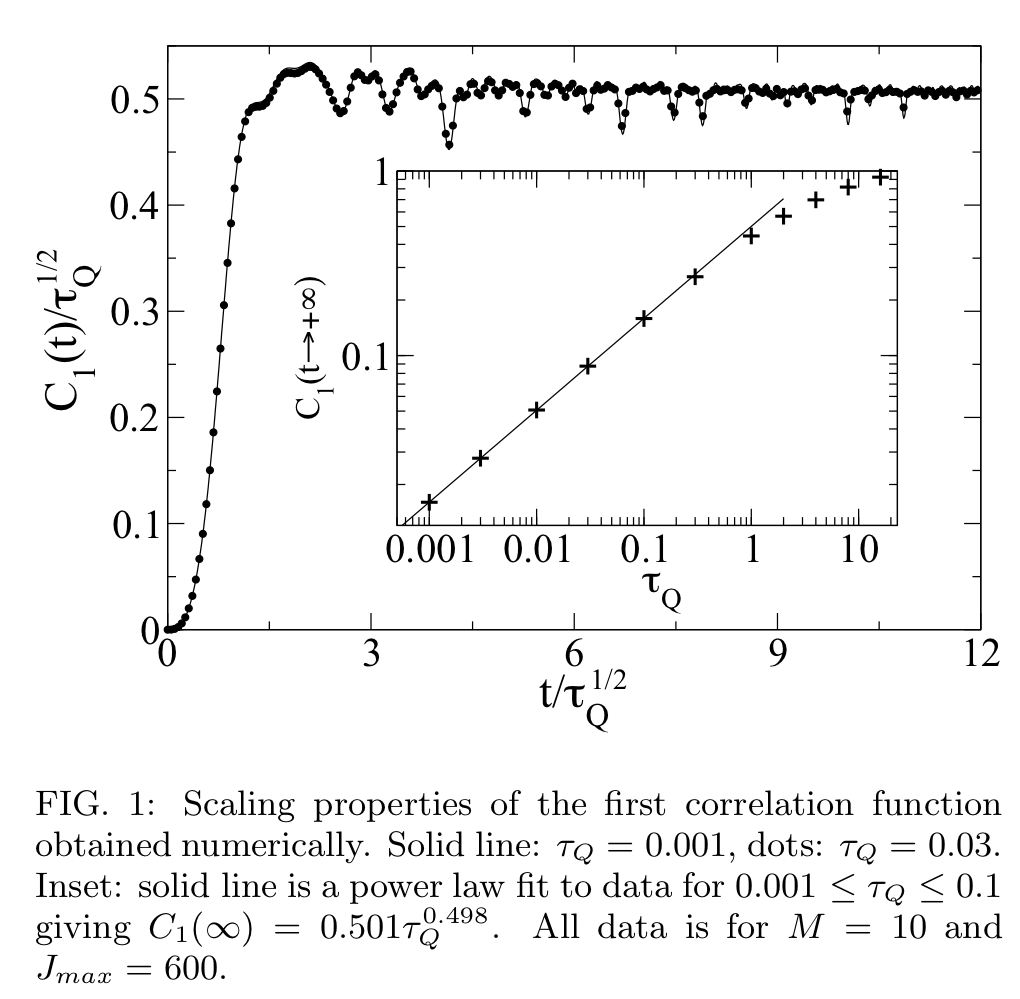
\includegraphics[width=10cm]{SSP3_1.png}
  \caption{$M=10, J_{\mathrm{max}}=600$としたモデルの計算結果.外側の図は$C_1(t)$のスケーリング則を示しており,実線は$\tau_Q=0.001$,点は$\tau_Q=0.03$の計算結果である.内側の図はフィッティングの結果を示しており,実線は$C_1(\infty) = 0.501\tau_Q^{0.498}$の直線である.}
  \label{fig:paper_1}
\end{figure}

次に,著者らは上述した結果を(1)時間に依存する摂動論と(2)ボゴリューボフ理論を用いて説明していた.
ここでは(1)を中心に解説し,(2)については結果だけ書く.

まず,$M>2$を仮定して,波動関数を
\begin{equation}
  \ket{\psi(t)} = a(t) \ket{1,1,\cdots} + \frac{b(t)}{\sqrt{2M}} \left(\ket{0,2,1,\cdots} + \ket{2,0,1,\cdots} + \ket{1,0,2,1,\cdots} + \ket{1,2,0,1,\cdots} \cdots \right)
\end{equation}
と書く.
ただし,$\left|a(t)\right|^2+\left|b(t)\right|^2=1$とする.
このとき,時間に依存する摂動論から,$a(t),b(t)$は
\begin{equation}
  i\dv{t} 
  \left(
  \begin{array}{c}
    a(t) \\
    b(t) \\
  \end{array}
  \right)
  = \left(
  \begin{array}{cc}
    0 & -2\sqrt{M}\frac{t}{\tau_Q}\\
    -2\sqrt{M}\frac{t}{\tau_Q} & 1\\
  \end{array}
  \right)
  \left(
  \begin{array}{c}
    a(t) \\
    b(t) \\
  \end{array}
  \right)
\end{equation}
と時間発展することが分かる.
基底を変換し,ランダウ-ツェーナー(LZ)モデルと対応づけて$C_1(t)$を導出し,それを$\tau_Q \ll 1$として展開すると結局
\begin{equation}
  \frac{C_1(t)}{\sqrt{\tau_Q}} = \frac{2}{3}\left[\frac{t}{\sqrt{\tau_Q}}\right]^{3} \label{c1}
\end{equation}
が分かる.
詳細は省くが,ボゴリューボフ理論で導かれる式の展開式の第1項はこの式と合致する.
また,ボゴリューボフ理論を用いると,一般の$l$について$C_l(t)$が導出できる.

この結果を$M=10$の場合に数値計算と比較すると,図\ref{fig:paper_2}のようになる.
このことから,$t/\sqrt{\tau_Q} < 0.5$でこの結果は数値計算と合っていることが分かる.

\begin{figure}[htbp]
  \centering
  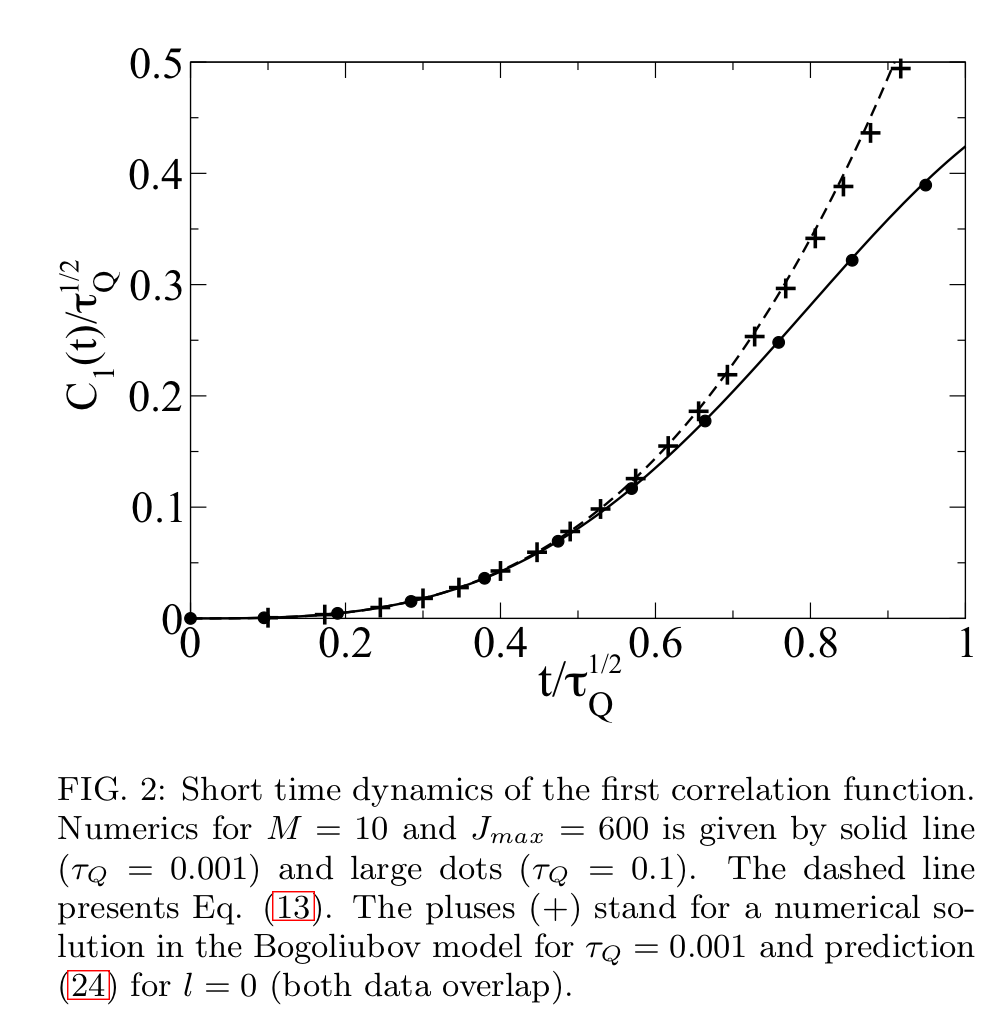
\includegraphics[width=10cm]{SSP3_2.png}
  \caption{$C_1(t)$の短時間のダイナミクス.実線と大きな点は$M=10, J_{\mathrm{max}}=600$としたモデルで$\tau_Q=0.001$,$\tau_Q=0.1$としたときの計算結果.破線は時間に依存する摂動論で得られる式\eqref{c1}を表す.プラス($+$)は,ボゴリューボフ理論による計算結果($\tau_Q=0.001$).$t/\tau_Q < 0.5$では摂動論もボゴリューボフ理論も数値計算結果とよく一致する.}
  \label{fig:paper_2}
\end{figure}

\subsection*{感想}
今まで物性理論をしっかり勉強したことがなかったのであまり深掘りできませんでしたが,非常に良い経験になりました.
内容について言えば,スケーリング則の有用性を実感しました.
自分がこれから専門にするソフトマター(または生物物理)の領域でも,de Genneのような研究者がスケーリング則を用いて高分子の議論をしていたので,スケーリングの感覚は大切に持っておきたいと思います.

\end{document}